\documentclass[11pt]{report}
\usepackage{graphicx}
\usepackage{amsmath}
\usepackage{subfigure}
\usepackage{caption}
\usepackage{subcaption}
%opening
\title{Assistive Technologies for the Visually Impaired}
\author{Ameya A. Joshi\\Department of Electrical and Electronics\\ BITS Pilani KK Birla Goa Campus\\f2010005@goa.bits-pilani.ac.in
\and
 G.A. Pavan Kumar\\
 Department of Electronics and Communications\\
 BITS Pilani Hyderabad Campus\\
 f2010018@hyderabad.bits-pilani.ac.in}

\begin{document}

\maketitle

\begin{abstract}
We provide a description of the research  and development process of \textbf{LeChal}, an navigational shoe for the visually impaired. The report discusses the various subsystems concentrating the obstacle avoidance system. We provide an in depth look at the theory and implementation of the Sonar and 3D vision based navigation system along with a brief overall view of the complete system. We also give examples of the various use cases and a few trial examples. The prototype uses stereo correspondence using BRIEF\cite{brief} descriptors and BruteForce matching using the L2 norm in order to calculate the disparity map in order to provide the depth values. We then use a homography based algorithm to calculate the height of an obstacle\cite{obstacleavoidance}. The prototype supplements this data with a Sonar reading to detect an obstacle and provide feedback using a vibrational motor. The prototype gives very accurate results in the controlled environments tested so far. Further testing is to be done in conjunction with the LV Prasad Eye Institute, Hyderabad to get clinical certification.     
\end{abstract}
\tableofcontents
\listoffigures
\chapter{Introduction}
A recent study conducted by WHO\cite{who} revealed that there are more than 800 Million visually impaired people in the world. Out of these, 90\% live in  developing countries 
where in there are not enough facilities for treatment and rehabilitation. In view of these horrifying statistics, LeChal\cite{lechal}, our flagship product proves to be a great boon to those who cannot see the world as we do.  

\textbf{LeChal}, in essence, is a haptic feedback based navigation device embedded in footwear. Haptic, here, refers to a one of a kind, easy to learn vibrational language which allows the visually impaired to know about their surroundings and navigate as efficiently and safely as possible. The innovation displayed by the product is the ease of use with which navigational cues are conveyed to the users. 

This project attempts at integrating a computer vision system using stereo vision.Stereo Vision\cite{gonzalez,HOGDisp} involves using multiple images to get 3D information from the image. In this application, we use two images taken from cameras with parallel optical axes. The system uses the 3D information from the two images to analyze the presence and size of the obstacles.In order to test out our algorithm, we have constructed a prototype and have managed to test it successfully under controlled conditions. The code has also been ported successfully to Android using OpenCV4Android\cite{Opencvandroid} and is being clinically and technically tested. 

This report documents the various techniques that we use for the above as well as the technical specifications and use cases for the prototype. The report has been structured as follows. The first chapter deals with a brief overview of the problem and a discussion on the existing technologies. We follow this by describing the methodology used in the solution we describe. We then discuss the entire algorithm briefly in a few use cases in the next chapter. This is followed by a brief conclusion and plans for future work regarding this project. 

We will now discuss related work being conducted in this field and provide a brief introduction to the solutions provided by the wider research community.



\section{Related Work}

There have been several approaches towards creating navigational aids for the visually impaired. Helal et al\cite{helal2001drishti,ran2004drishti} have created Drishti, an indoor/outdoor navigation system for the visually impaired using Geographic Information Systems,GPS and wearable technology.They leverage it as a wearable computer which provides voice feedback for navigation. The problems with this approach are that it is more technology centric rather than user centric. Most visually impaired people are not comfortable with a computer though the figure of those who are is increasing rapidly. 

NAVI, a Kinect based indoor navigation system\cite{Zollner20118609458}, was proposed by Z\"{o}llner et al. as an 3D mapping navigational system with vibrational feedback. Their prototype, however was not integrated into anything wearable and was not unobtrusive, also being cost prohibitive. Smart Cane \cite{sakhardande2012smart} was developed using ultrasound ranging technology. It too provides vibrational feedback in proportion with the distance to the obstacle.

BlindSquare\cite{blindsquare} is an iPhone app which uses the online location sharing site, FourSquare in addition to the phone's own GPS system to provide cues for travelling. This though will not provide real-time information about the environment.      

Several other systems exist providing navigational data through either vibration or audio feedback based on the principles discussed before. 

The major difference between the above mentioned technologies and our product is the unobtrusive nature of our product. A user is not particularly marked out because of some bulky and highly visible device or due to obvious cues in the form of audio. We rely on the fact that every person will wear shoes and can feel the haptic cues from the device. The cues being highly natural will also not require him to spend time training. 

Another major advantage of using shoes is they give a good vantage point for the cameras to detect dangerous obstacles at a reasonable distance. We aim to detect obstacles within ranges of 3-5 metres and the cameras provide a more than reasonable view of that distance. 

The greatest advantage over all the above systems is that uses and enhances the existing technologies available. With the shoes connecting to any available Android phone, it does not require bulky attachments or a lot of power. Thus, the product become unobtrusive, easy to use and highly intuitive.  

We give a general overview of the LeChal system and a brief description of technologies available in the following section.   

\section{Overview}
Visual Impairment is currently a major disability in the world affecting a large part of the population\cite{who}. In spite of this, a large percentage of our day to day life is spent interacting with objects which are meant to be seen, understood and acted upon. A major problem faced by the visually impaired community is navigation, especially, urban navigation. 

Navigation is a very complex problem to deal with as humans in general use all of their senses for the same. In particular, sight provides a large impetus for localization and avoidance of obstacles. Thus, loss of sight creates a huge void in the way the visually impaired navigate. In such a case, computer vision is a very intuitive way to solve this problem by providing the missing information about one's environment.

Computer vision has long been used for navigation in robots and autonomous vehicles\cite{nav1,nav2}. There are various techniques that have been used including obstacle detection using single camera\cite{nav2}, SLAM\cite{slam} and  stereovision\cite{stereo1,outdoorstereo,murray1997stereo,murray2000using}. It involves getting data about the environment and analyzing it to get a sense of the terrain around the camera. 

The primary challenges for this approach are
\begin{itemize}
	\item The obstacle has to be segmented from the background
	\item The algorithm must work real time
	\item The algorithm must be robust enough to work in a fairly complex environment
\end{itemize}

Stereo-Vision provides solutions to all the above challenges successfully. Labayrade et al.\cite{labayrade2002} provides a very good example of using stereo-vision for navigation in a real-time environment. Our algorithm uses optimized versions of the technique used in the above paper and Rahman's thesis\cite{obstacleavoidance} and  deals with all these challenges in a new and robust way. We have also customized the entire algorithm to work in conjunction with a secondary SONAR system. 

SONAR has always been used a navigational aid for several applications including submarines, fishing vessels and in other such low visibility environments. We use SONAR for corroborating and enhancing the navigational data we get from our stereo-vision system. Elfes\cite{sonar} in his paper on using SONAR for realtime navigation provides a brilliant example. 

Using SONAR and stereo-vision along with an accelerometer and magnetometer based step detection system, we are able to provide a fairly accurate system for providing low level navigational cues to avoid obstacles and create an indoor mapping system. We have modified this entire system to be placed into a shoe so that the system is unobtrusive and very intuitive to use.


\section{LeChal-Systems and Integration}

As presented above, various different systems exist for navigation of the visually impaired. In this section, we discuss the approach we use for \textbf{LeChal} and the various improvements it makes on the existing system. We also give a brief description of our contribution to the existing system.

LeChal, basically consists of three high level systems:
\label{subsystems}
\begin{itemize}
\item High Level Navigation
\item Low Level Navigation 
\item Obstacle and Terrain Detection
\item Feedback and Communication
\end{itemize}

Each of these high level systems consist of several subsystems in order to achieve the required objective. 

We will now discuss the various subsystems in some detail.

\subsection{High Level Navigation}

The primary aim of the high-level navigation system is to help the visually impaired from one place to the other. LeChal achieves this through the use of the GPS system in an Android phone. 

The basic premise of GPS is that it uses global positioning satellites situated around the earth to triangulate their location using the time required by the radio signals to reach the GPS receiver\cite{gps}. A GPS receiver's job is to locate four or more of these satellites, figure out the distanc­e to each, and use this information to deduce its own location. This operation is based on a simple mathematical principle called trilateration. 

In order to make this simple calculation, then, the GPS receiver has to know two things:
\begin{itemize}
\item The location of at least three satellites above you
\item The distance between you and each of those satellites
\end{itemize}

The GPS receiver figures both of these things out by analyzing high-frequency, low-power radio signals from the GPS satellites. Better units have multiple receivers, so they can pick up signals from several satellites simultaneously.

Radio waves are electromagnetic energy, which means they travel at the speed of light (about 186,000 miles per second, 300,000 km per second in a vacuum). The receiver can figure out how far the signal has traveled by timing how long it took the signal to arrive. 

These GPS co-ordinates in conjunction with Google APIs for allowing the user to easily access his current position and give the system the location of the place he wants to travel to. With recent updates in Google APIs, we have the opportunity to even integrate transit information like bus stops and bus numbers to allow for greater flexibility in travel. The entire GPS system works on the Android phone using the Android SDK. The communication between the shoe and the phone is provided through a bluetooth connection which will be discussed further on in the future sections.

\begin{figure}[hp]
\centering
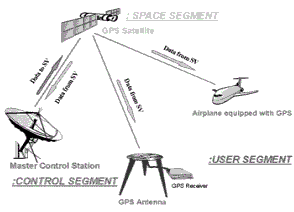
\includegraphics[scale=0.5]{fig1.png}
\caption[Different parts of GPS System]{Different parts of GPS System}
\end{figure}

\subsection{Low Level Navigation}

GPS systems provide a very accurate way of navigating from pt. A to pt. B. But, to provide proper navigational cues, several other parameters like orientation and direction need to be taken into account. With respect to this, we use an electronic system with an accelerometer and a magnetometer. 

The accelerometer provides acceleration values along the three axes, X, Y and Z, with respect to itself. The acceleration output provides a way to calculate the approximate position and velocity of the moving foot. This is being used to calculate footsteps and there on in indoor navigation. 

The magnetometer is a 3-axis electronic compass which gives quantized values of the direction with respect to the magnetic north pole. This is then used for the calculation of orientation and the correction required to put the user on the correct path. This entire system communicates with phone and makes decisions with regards to the GPS co-ordinates of the user and the destination. 

The product thus ensures that the user is able to navigate from a source location to a destination location in a timely manner. But in order to give more information to him about the environment, we have created an obstacle avoidance system which is the crux of this document.

\subsection{Obstacle and Terrain Detection}

In any environment, safe navigation requires to know the position and the type of teh obstacles in our path. We achieve this in LeChal by using a combination of Stereovision and Sonar. 

Stereovision is a field of computer vision which involves using views from multiple angles to get data about the 3D position of a point. The basic principle of stereovision is triangulation- that is, using the projections of a point in 3D space on 2 different images to obtain an estimate of its location in 3D space. We use binocular disparity in achieving this. We then use the concept of 3D reconstruction\cite{hartley2000multiple} to get approximate locations of obstacles.

Stereo vision may fail sometimes due to a low frequency image or a fast moving objects. In such a case, we propose to use a SONAR system to supplement the stereovision system.SONAR(Sound Navigation and Ranging) or ultrasonic sensing uses propagation of acoustic energy at higher frequencies than normal hearing to extract information from the environment.This technique can be used to navigate ,communicate with or detect objects.Matthies and Elfes\cite{sonarstereo} implement a similar system for path planning using grid representation. Since we are only dealing with close range obstacles, we use a simpler version of the algorithm along with Rahman's homography based method\cite{obstacleavoidance} to create a failsafe system. 

We integrate this entire system to only react when the foot is stationary on the ground by using a pressure sensor to trigger it. This allows for an optimum version of obstacle detection allowing for enough time for processing the incoming images.

In this report, we will be primarily discussing our contribution to the stereovision system and our experiments regarding integrating the various subsystems into a working prototype for testing.

This entire system requires accurate signaling from the various systems as well as a powerful platform for control. In the next section we discuss the feedback and communications part along with the overall control structure.

\subsection{Feedback and Communication}

As discussed in the earlier sections, we require a fairly fast and accurate system of signaling for control and integration. With most modern phones supporting bluetooth and the backbone of the entire system being an Android phone, the system uses bluetooth to transmit and receive information between the various sub-systems. 

The earlier models of LeChal used bluetooth for signaling and transmitting directional and orientation data\cite{compdata}. We have expanded the system to process and transmit images from the cameras on the shoe to the phone using bluetooth. We also propose a Wi-Fi based solution involving creation of a local network for faster transfer of data. 

The images are processed on the phone using OpenCV libraries and a signals are given to the micro-controller on the shoe regarding data about the obstacles in the Field of View(FoV).   
\newline
\newline
In the concluding section for this chapter, we discuss our primary contribution to the project and give a brief description of the structure of the report.

\section{Contribution}

In this section, we discuss our contribution towards the project and describe the structure of the report for ease of access.  

As discussed earlier in Section \ref{subsystems}, we have four major subsystems in the prototype. Our major contribution to the project is mainly regarding the Obstacle Detection system and the feedback and communication system. 

The existing codebase for stereovision was overhauled and optimized. It was also ported to Android. Experiments were conducted to ensure viable processing speeds on the phone processor to ensure real-time, seamless detection of obstacles and changes in terrain. 

The hardware for the prototype was researched for and finalized. This included the camera modules and the communication system module. The two subsystems were then integrated into the existing prototype and are being tested with the Android based platform. Currently, experiments are being conducted to test the viability of bluetooth as a method for communication with regards to the constraints of time. 

We also provided valuable inputs to the design team on technologies to create a user friendly design. 
\newline
\newline
The following chapters provide in depth information about our methodology and the hardware and software used. We will be discussing the various methodologies followed for prototyping as well as the subsystems of Obstacle Detection and Feedback and Communication in detail. We follow this by providing a high level description of the prototype itself. The final chapter provides a plan for future work regarding this project. In this report, we mainly deal with the Obstacle detection subsystem and the communication protocols used to convey data to and from the device.

The next chapter discusses the methodology of our project along with a detailed discussion on the two subsystems mentioned in the previous sections.

\chapter{Methodology}

The primary use case of LeChal is as a navigational aid for the visually impaired. This requires us to have a highly accurate results in case of obstacle detection and a well tuned navigation system with multiple redundancies while being power efficient for portability. With all these constraints taken into consideration, we primarily use an existing piece of technology owned by almost everybody - a smart phone. With the recent advent of smart phones and the highly popular Android Operating system, it is an easy choice to use the phone's processing power to make the shoes themselves less bulky.

Our contribution to the project was to develop the obstacle avoidance system. This basically involved two major objectives.

\begin{itemize}
\item SONAR based navigation
\item Camera control and Image Transfer to the phone
\item Stereo Vision Processing on the phone
\end{itemize}        

In the following sections, we will discuss the above problem statements in greater detail as well as the various methods we use to solve them.

\section{Bluetooth transfer of the images}

Our primary plan of action was to design an on-board system for the shoe. We decided to use the already existing platform of an android phone in order to reduce the burden of costs on the customer as well as make the system easier to integrate in the confines of a shoe. For this we decided to proceed with sending the images to the phone through bluetooth. For our prototype, we used an existing arduino based solution which uses a shield known as ARDUCAM to transfer the high speed data from the camera, byte by byte, to the phone. 

The advantage of using bluetooth over other channels of communication is the low power requirement as well as the low cost of the modules themselves. We use the SPP profile of the bluetooth stack available in android phones by default. It emulates a normal serial port through which we can send data byte by byte. 

We have implemented  the above system using the ARDUCAM shield and the Arduino.

Arduino is a single-board microcontroller to make using electronics in multidisciplinary projects more accessible. The hardware consists of an open-source hardware board designed around an 8-bit Atmel AVR microcontroller, or a 32-bit Atmel ARM. The software consists of a standard programming language compiler and a boot loader that executes on the microcontroller. 

Official Arduinos have used the megaAVR series of chips, specifically the ATmega8, ATmega168, ATmega328, ATmega1280, and ATmega2560. A handful of other processors have been used by Arduino compatibles. Most boards include a 5 volt linear regulator and a 16 MHz crystal oscillator (or ceramic resonator in some variants), although some designs such as the LilyPad run at 8 MHz and dispense with the onboard voltage regulator due to specific form-factor restrictions. An Arduino's microcontroller is also pre-programmed with a boot loader that simplifies uploading of programs to the on-chip flash memory, compared with other devices that typically need an external programmer.

At a conceptual level, when using the Arduino software stack, all boards are programmed over an RS-232 serial connection, but the way this is implemented varies by hardware version. Serial Arduino boards contain a level shifter circuit to convert between RS-232-level and TTL-level signals. Current Arduino boards are programmed via USB, implemented using USB-to-serial adapter chips such as the FTDI FT232. Some variants, such as the Arduino Mini and the unofficial Boarduino, use a detachable USB-to-serial adapter board or cable, Bluetooth or other methods. (When used with traditional microcontroller tools instead of the Arduino IDE, standard AVR ISP programming is used.)

As the Arduino is a low power, low speed microcontroller, we need to use a separate interface in order to send the high speed camera data through the bluetooth serial channel. For this, we use the ARDUCAM shield. In simple terms, the ARDUCAM shield acts as a buffer between the camera and the Arduino, so as to store the data from the camera before sending it serially through bluetooth.

ArduCAM is an open source project for CMOS camera modules, which hide the complexity of capturing high speed high resolution image data stream and provide the source code configuration for camera modules. User can freely control the ArduCAM shield to accomplish their different tasks.

The use cases of ArduCAM include:

\begin{itemize}
\item Capture still images
\item Real time preview on 3.2” LCD screen
\item Wireless image transmission
\end{itemize}

We use the ArduCAM shield for wireless transmission of images through the use of an external bluetooth device. We use the HC-06 module for this. HC-06 is a fairly popular, low cost bluetooth slave module. It supports high speed bluetooth communication along with several bluetooth profiles like SPP, A2DP etc.

We will now discuss the bluetooth based communication system that we have used in our product.
\section{Bluetooth}
The Android platform includes support for the Bluetooth network stack, which allows a device to wirelessly exchange data with other Bluetooth devices. The application framework provides access to the Bluetooth functionality through the Android Bluetooth APIs\cite{androiddevguide}. These APIs let applications wirelessly connect to other Bluetooth devices, enabling point-to-point and multipoint wireless features.
Using the Bluetooth APIs, an Android application can perform the following:

\begin{itemize}
\item Scan for other Bluetooth devices
\item Query the local Bluetooth adapter for paired Bluetooth devices
\item Establish RFCOMM channels
\item Connect to other devices through service discovery
\item Transfer data to and from other devices
\item Manage multiple connections
\end{itemize}

We will now discuss the Bluetooth API of the Android SDK.
 
\subsection{Basics of Bluetooth} 

This section describes how to use the Android Bluetooth APIs to accomplish the four major tasks necessary to communicate using Bluetooth: setting up Bluetooth, finding devices that are either paired or available in the local area, connecting devices, and transferring data between devices.
All of the Bluetooth APIs are available in the android.bluetooth package. Here's a summary of the classes and interfaces you will need to create Bluetooth connections:
\begin{enumerate}

\item \textbf{BluetoothAdapter}\newline 
Represents the local Bluetooth adapter (Bluetooth radio). The BluetoothAdapter is the entry-point for all Bluetooth interaction. Using this, you can discover other Bluetooth devices, query a list of bonded (paired) devices, instantiate a BluetoothDevice using a known MAC address, and create a BluetoothServerSocket to listen for communications from other devices.
\item \textbf{BluetoothDevice}\newline 
Represents a remote Bluetooth device. Use this to request a connection with a remote device through a BluetoothSocket or query information about the device such as its name, address, class, and bonding state.
\item \textbf{BluetoothSocket}\newline 
Represents the interface for a Bluetooth socket (similar to a TCP Socket). This is the connection point that allows an application to exchange data with another Bluetooth device via InputStream and OutputStream.
\item \textbf{BluetoothServerSocket}\newline 
Represents an open server socket that listens for incoming requests (similar to a TCP ServerSocket). In order to connect two Android devices, one device must open a server socket with this class. When a remote Bluetooth device makes a connection request to the this device, the BluetoothServerSocket will return a connected BluetoothSocket when the connection is accepted.
\item \textbf{BluetoothClass}\newline 
Describes the general characteristics and capabilities of a Bluetooth device. This is a read-only set of properties that define the device's major and minor device classes and its services. However, this does not reliably describe all Bluetooth profiles and services supported by the device, but is useful as a hint to the device type.
\item \textbf{BluetoothProfile}\newline 
An interface that represents a Bluetooth profile. A Bluetooth profile is a wireless interface specification for Bluetooth-based communication between devices. An example is the Hands-Free profile. 
\item \textbf{BluetoothHeadset}\newline 
Provides support for Bluetooth headsets to be used with mobile phones. This includes both Bluetooth Headset and Hands-Free (v1.5) profiles.

\item \textbf{BluetoothA2dp}\newline 
Defines how high quality audio can be streamed from one device to another over a Bluetooth connection. "A2DP" stands for Advanced Audio Distribution Profile.

\item \textbf{BluetoothHealth}\newline 
Represents a Health Device Profile proxy that controls the Bluetooth service.

\item \textbf{BluetoothHealthCallback}\newline 
An abstract class that you use to implement BluetoothHealth callbacks. You must extend this class and implement the callback methods to receive updates about changes in the application’s registration state and Bluetooth channel state.

\item \textbf{BluetoothHealthAppConfiguration}\newline 
Represents an application configuration that the Bluetooth Health third-party application registers to communicate with a remote Bluetooth health device.

\item \textbf{BluetoothProfile.ServiceListener}\newline 
An interface that notifies BluetoothProfile IPC clients when they have been connected to or disconnected from the service (that is, the internal service that runs a particular profile)

\end{enumerate}

The next section deals with the requirements and implementation of the bluetooth subsystem of our project.

\label{imagetransfer}
\subsection{Image Transfer}

\label{stereoalgo}
\section{Stereo Vision for obstacle avoidance}

In obstacle avoidance, a major problem is to gauge the height and position of the obstacle in three-dimensional space. There are various electronic, mechanical and computational methods to achieve this\cite{slam,infrared, thorpe1988vision}. Our major advantage in this case is that a person may use his other senses also to navigate using the cues from the shoe only as suggestions. Hence, our system though accurate does not need to be pinpoint accurate as robotic vehicle might need to be.

In order to optimise the system for such a use case, we decided to use stereovision\cite{gonzalez,hartley2000multiple} in order to implement our obstacle detection algorithm. 

Marr et al\cite{marr1991computational} in their seminal paper on human stereo vision, present a computational method to determine depth from images from multiple viewpoints similar to how the human brain does it. Grimson and Leifur \cite{grimson1981computer} provided an expanded version of Marr's theory as well as an implementation of the same.

Current state-of-the-art stereo-vision techniques\cite{taxonomy} all expand Grimson's technique of dense stereo correspondence using feature matching in order to get a dense disparity map. The dense disparity map can then be reprojected with camera matrices into a three dimensional scene. In our algorithm, we stop at the dense disparity map extraction in order to save on computation.

For our stereovision subsystem, we follow the following steps:

\begin{enumerate}
\item Camera Calibration
\item Stereo Calibration
\item Dense Stereo Correspondence
\item Approximation of the height of detected obstacles
\end{enumerate} 

We will discuss the each of the above steps in detail in the following sub sections.
\label{calib}
\subsection{Calibration}

Cameras have been around for a long-long time. However, with the introduction of the cheap pinhole cameras in the late 20th century, they became a common occurrence in our everyday life. Unfortunately, this cheapness comes with its price: significant distortion. Luckily, these are constants and with a calibration and some remapping we can correct this. Furthermore, with calibration you may also determine the relation between the camera’s natural units (pixels) and the real world units (for example millimeters). 

For calibration, we basically need to solve a few equations to get the transformations

\begin{equation}
x_{corrected} = x(1+k_{1}r^{2}+k_{2}r^{4}+k_{3}r^{6})
\end{equation}


\begin{equation}
y_{corrected} = y(1+k_{1}r^{2}+k_{2}r^{4}+k_{3}r^{6})
\end{equation}

So for an old pixel point at ${(x,y)}$ coordinates in the input image, its position on the corrected output image will be ${(x_{corrected}, y_{corrected})}$. The presence of the radial distortion manifests in form of the “barrel” or “fish-eye” effect.

Tangential distortion occurs because the image taking lenses are not perfectly parallel to the imaging plane. It can be corrected via the formulas:
\begin{equation}
x_{corrected} = x + [2p_{1}xy + p_{2}(r^{2} + 2x^{2})] 
\end{equation}

\begin{equation}
y_{corrected} = y + [p_{1}(r^{2} + 2x^{2}) + 2p_{2}xy] 
\end{equation}

So we have five distortion parameters which in OpenCV are presented as one row matrix with 5 columns:

$Distortion_{coefficients}=(k_1 \hspace{10pt} k_2 \hspace{10pt} p_1 \hspace{10pt} p_2 \hspace{10pt} k_3)$

Now for the unit conversion we use the following formula:
\begin{equation}
\begin{bmatrix}
x \\ y \\w
\end{bmatrix}=
\begin{bmatrix}
f_x & 0 & c_x\\
0 & f_y & c_y\\
0 & 0 & 1
\end{bmatrix}
\begin{bmatrix}
X \\ Y \\ Z
\end{bmatrix}
\end{equation}


Here the presence of w is explained by the use of homography coordinate system (and w=Z). The unknown parameters are $f_x$ and $f_y$ (camera focal lengths) and $(c_x, c_y)$ which are the optical centers expressed in pixels coordinates. If for both axes a common focal length is used with a given a aspect ratio (usually 1), then $f_y=f_x*a$ and in the upper formula we will have a single focal length f. The matrix containing these four parameters is referred to as the camera matrix. While the distortion coefficients are the same regardless of the camera resolutions used, these should be scaled along with the current resolution from the calibrated resolution.

The process of determining these two matrices is the calibration. Calculation of these parameters is done through basic geometrical equations. The equations used depend on the chosen calibrating objects. Currently OpenCV supports three types of objects for calibration:

\begin{itemize}
 \item Classical black-white chessboard
 \item Symmetrical circle pattern
 \item Asymmetrical circle pattern
\end{itemize}

Basically, you need to take snapshots of these patterns with your camera and let OpenCV find them. Each found pattern results in a new equation. To solve the equation you need at least a predetermined number of pattern snapshots to form a well-posed equation system. This number is higher for the chessboard pattern and less for the circle ones. For example, in theory the chessboard pattern requires at least two snapshots. However, in practice we have a good amount of noise present in our input images, so for good results you will probably need at least 20 good snapshots of the input pattern in different positions.

Here are two of the example input and undistorted images:



\begin{figure}
\centering
\parbox{5cm}{
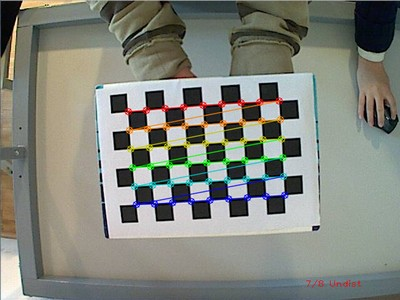
\includegraphics[width=5cm]{normal.jpg}
\caption{Left Image}
\label{fig:2figsA}}
\qquad
\begin{minipage}{5cm}
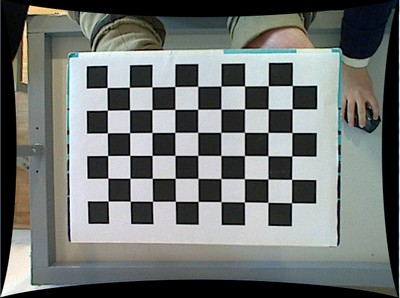
\includegraphics[width=5cm]{undist.jpg}
\caption{Disparity map}
\label{fig:2figsB}
\end{minipage}
\end{figure}

We will now take a look at the stereo calibration module of the project
\newpage
\subsection{Stereo Calibration}
Stereo calibration is similar to single camera calibration but it involves more steps and gives complete intrinsic and extrinsic parameters. 

\begin{equation}
sm' = A[R|t]M'
\end{equation}

This can also be represented in the following way,

\begin{equation}
s\begin{bmatrix}
u \\ v \\1
\end{bmatrix}
=\begin{bmatrix}
f_x & 0 & c_x\\
0 & f_y & c_y\\
0 & 0 & 1
\end{bmatrix}
\begin{bmatrix}
r_{11} & r_{12} & r_{13} & t_1\\
r_{21} & r_{22} & r_{23} & t_2\\
r_{31} & r_{32} & r_{33} & r_3\\

\end{bmatrix}
\begin{bmatrix}
X \\ Y \\ Z \\ 1
\end{bmatrix}
\end{equation}

where:
\begin{itemize}



  \item      $(X, Y, Z)$ are the coordinates of a 3D point in the world coordinate space
  \item      $(u, v)$ are the coordinates of the projection point in pixels
  \item      $A$ is a camera matrix, or a matrix of intrinsic parameters
  \item      $(cx, cy)$ is a principal point that is usually at the image center
  \item      $fx, fy$ are the focal lengths expressed in pixel units.

\end{itemize}

We get $A$ from our calibration as described in \ref{calib}. We can then use the same method of getting pairs of chessboard images of various orientations and positions to solve for the remaining transforms. We have used OpenCV's existing stereoCalibrate method to find out the $R$ and $t$ matrices\cite{opencvdoc} 

The function estimates transformation between two cameras making a stereo pair. If you have a stereo camera where the relative position and orientation of two cameras is fixed, and if you computed poses of an object relative to the first camera and to the second camera, $(R_1, T_1)$ and $(R_2, T_2)$, then those poses definitely relate to each other. This means that, given $( R_1,T_1 )$, it should be possible to compute $( R_2,T_2 )$. You only need to know the position and orientation of the second camera relative to the first camera.

The next part of our report will explain the dense correspondence methodology in order to get the final disparity maps for the depth information.

\newpage
\label{steroc}
\subsection{Dense Stereo Correspondence}

With the matrices calculated in the earlier sections, we can get accurate 3D estimation from images taken from the stereo setup. But the images also need to be aligned and , we need to know which pixels from the left image correspond to the pixels from the right in order to get a disparity map. 

Disparity maps are simply maps of the difference in either $X$ or $Y$ axis of corresponding pixels in a pair of images that we get from the stereo cameras. As such, we need to find the correspondence of the said pixels. There are a no. of methods using various features to get the dense stereo correspondence, but we use the Semi Global Block Matching method(SGBM)\cite{hirschmuller2008stereo} along with BRIEF features\cite{brief} to get the stereo correspondence.

Our implementation uses FAST corner detection\cite{rosten_2006_machine} along with BRIEF descriptors to get feature points for the pair of images from the stereo camera. We then match the feature descriptors from the two images using a Brute Force L1 norm based matcher. We then calculate the disparity map using the SGBM method. 



\begin{figure}
\centering
\parbox{5cm}{
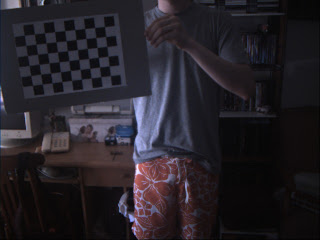
\includegraphics[width=5cm]{left.jpg}
\caption{Left Image}
\label{fig:2figsA}}
\qquad
\begin{minipage}{5cm}
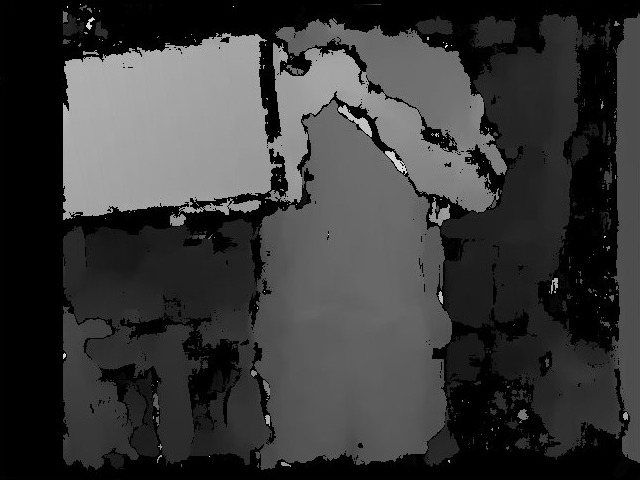
\includegraphics[width=5cm]{disp.jpg}
\caption{Disparity map}
\label{fig:2figsB}
\end{minipage}
\end{figure}




In the disparity map, the closer objects are brighter in intensity while the farther ones are darker. The black parts of the image are where the disparity could not be calculated. The disparity map can be further processed with anisotropic or bilateral filters to get more accurate results. We do not use any filters as we require this to be realtime and as fast as possible. 

In order to optimise for speed, we have changed our approach a bit by only calculating the 20 best feature matches and only calculating SGBM based disparities for them. This gives us accurate enough results without being time consuming. 

\label{height}
\subsection{Approximation of the height of the detected obstacle}

From the earlier section, we get feature descriptors and disparity values corresponding to the 20 best feature points. Using the fact that lower disparity values correspond to closer objects, we get the closest objects to the cameras. We then use the homography based method described in Rahman's thesis\cite{obstacleavoidance} to estimate the height of the detected objects. We describe the method in the following paragraphs.

In order to estimate the height of each point, it is necessary to know the homography of the plane it corresponds to. So, homographies of each plane at intervals of one distance unit (cm) are computed using the standard homography formula for parallel planes using $h_matrix$ as H from distance = camera height (ch) and $h_inf$ as H from distance = infinity. We assume $h_inf$ to be an identity matrix given that points at infinity hardly seem to move when the image is warped. 

The basic premise of the method is to find how much a point's position changes when it is projected from its height to the floor. Using this projection, we can decide the height. We calculate the homographies of each point using the following equation:

\begin{equation}
H_{point} = H_{matrix}(c_h/h_t) + h_{inf}(1-(c_h/h_t))
\end{equation}
 

In order to estimate the height of a point $(i_x,i_y)$ on image-1 which has acorresponding point $(f_x,f_y)$ on image-2, $(ex,ey)$ is calculated for $(i_x,i_y)$ for each parallel plane at heights i = 0 to $c_h$ and a comparison is made between $(e_x,e_y)$ and $(f_x,f_y)$ using a distance measure. The height i selected as the estimated height for $(i_x,i_y)$ is the height at which using $h_{point}(i)$ the comparing variable $d$has the lowest value, i.e. the height at which the point $(i_x,i_y)$ seems to match the best.

We iterate through the various heights and use the following equations to calculate the height. 

\begin{equation}
\begin{bmatrix}
e_x \\ e_y \\ tmp 
\end{bmatrix}
= h_{matrix} * \begin{bmatrix}
i_x \\ i_y \\ 1
\end{bmatrix}
\end{equation} 

\begin{equation}
p = \sqrt{(i_x - e_x)^2 + (i_y + e_y)^2}
\end{equation} 

\begin{equation}
q = \sqrt{(f_x - i_x)^2 + (f_y + i_y)^2}
\end{equation} 

\begin{equation}
r = \sqrt{(f_x - e_x)^2 + (f_y + e_y)^2}
\end{equation} 

\begin{equation}
t = \cos(\frac{p^2+q^2-r^2}{2pq}) *\frac{180}{\pi}
\end{equation} 

\begin{equation}
d= \frac{100r}{q} + t
\end{equation}

If the value of $d$ is less than a minimum value, we return $i$ as the height of the object. We then use a simple thresholding mechanism to discard the features whose height is less than a certain threshold.

Thus we are able to use Stereoscopic vision to detect obstacles in the path of the user.

In the next section, we discuss the implementation of this system on the android phone using bluetooth to transfer images from the shoe mounted cameras to the phone.

\section{Implementation in OpenCV4Android}

In this section, we discuss our implementation of the methods discussed in section \ref{stereoalgo} using the OpenCV4Android SDK. 

Starting with 2.4.2 release for Android, OpenCV Manager is used to provide apps with the best available version of OpenCV. This involves using async inititalization which refers to dynamically adding the libraries to the app during runtime using the OpenCV Manager which is now an app on the Google Playstore\cite{playstore}.

\subsection{Application Development with Async Initialization}

Using async initialization is a recommended way for application development. It uses the OpenCV Manager to access OpenCV libraries externally installed in the target system.

In this case application works with OpenCV Manager in asynchronous fashion. OnManagerConnected callback will be called in UI thread, when initialization finishes. We have to note that it is not allowed to use OpenCV calls or load OpenCV-dependent native libs before invoking this callback. We can load your own native libraries that depend on OpenCV after the successful OpenCV initialization. Default BaseLoaderCallback implementations treat application context as Activity and call Activity.finish() method to exit in case of initialization failure.

The primary advantage of using Async Initialization is that the application size becomes small as libraries are later asynchronously loaded. This also helps in the application taking advantage of the latest updates to the library without requiring updates from the developer's side.

There are several disadvantages to this method too. AS all the functions requiring OpenCV are required to be implemented inside the BaseLoaderCallback, it is a bit tough to structure the code. Also, it requires the user to download a separate application to manage the OpenCV libraries itself.

\subsection{StereoVision in Android}

OpenCV4Android is the android port of the existing OpenCV library. Most functions of OpenCV have been implemented in this SDK using Java wrappers. 

The program starts with the transfer of images from the external stereo camera setup that we have discussed in \ref{imagetransfer}. These images are then passed to a function which implements the algorithm discussed in \ref{steroc} and \ref{height}. The entire algorithm has been implemented using the in-built functions of OpenCV along with a few custom functions for the height approximation.We started out with a C++ implementation for prototyping. We later on translated it to Android after optimising it for the same.

Two major challenges faced in the implementation of this system were:

\begin{enumerate}
\item The documentation of the OpenCV4Android was not adequate and thus, translating the code from the prototyped C++ code to the Androis code involved a lot of trial and error and implementation of bridging functions

\item The event based life cycle of Android apps had to be taken into consideration for the transfer of images and the procedural code implemented in OpenCV.
\end{enumerate}

To solve the above problems, we undertook a study of the OpenCV4Android SDK source code. We built several small example apps to implement separate parts of the c++ code. In order to sped up the appliation for android phones, we reduced the no. of feature points we considered to less than or equal to 20 which we landed on after experimenting with a dataset of images. 

\chapter{Conclusions}

In the preceding chapter, we have discussed the methodology of the entire system and the flow of the product. In this chapter, we will elaborate on the results of our tests on the prototype as well as the further work we plan to undertake. 



    

\bibliographystyle{ieeetr}
\bibliography{citation}
\end{document}

